\chapter{Lecture 04}

\begin{lem}[]\label{lemma01}
	Consider \( u\in L_{loc}^{p}(\Omega ;\mathbb{R}) \), with \( 1< p \leq  \infty  \) and fix \( \alpha \in \{ 1,2,\ldots,n \} \). The partial derivative \( \partial_{x_{\alpha }}u \) belongs to \( L_{loc}^{p}(\Omega ;\mathbb{R}) \) if and only if the family \( \Delta _{h,\alpha }u \) is uniformly bounded in \( L_{loc}^{p} \) as \( h \to 0 \).\\
	More precisely, if \( \forall \Omega' \ssubset \Omega \, \exists C=C(\Omega') \) such that
	\begin{gather}
		\abs{\int\limits_{\Omega'}^{} (\Delta _{h,\alpha }u) \varphi  \dd{x}}\leq c\norm{\varphi }_{L^{p'}(\Omega';\mathbb{R})} \qquad \varphi \in C_{c}^{1}(\Omega';\mathbb{R})
	\end{gather}
	with \( \frac{1}{p}+\frac{1}{p'}=1 \) and \( \abs{h}< \frac{1}{2} \operatorname{dist}(\Omega';\partial \Omega )  \).
\end{lem}
We now see how the previous lemma allows us to obtain regularity. We stick to the Poisson equation for the moment. \par
Suppose \( f \in H_{loc}^{1}(\Omega ;\mathbb{R})  \) and \( -\Delta u=f \) for some \( u \in H_{loc}^{1}(\Omega ; \mathbb{R})  \).\\
Being the equation translation invariant, we can write \( -\Delta (\tau _{h,\alpha }u) = \tau _{h, \alpha }f \), hence \( -\Delta (\Delta _{h, \alpha }u) = \Delta _{h, \alpha }f \) for any \( \Omega' \ssubset \Omega  \) and \( \abs{h}< \operatorname{dist}(\Omega', \partial \Omega )  \). \\
By Lemma~\ref{lemma01} it holds \( \Delta _{h, \alpha }f \) is bounded in \( L_{loc}^{2} \) uniformly in \( h \). By~\eqref{CLI} \( \abs{\nabla \Delta _{h, \alpha }U} \) is bounded in \( L_{loc}^{2}(\Omega ;\mathbb{R})  \), thanks to the Lemma~\ref{lemma01} (applied componentwise) we have that
\begin{gather}
	\partial_{x_{\alpha }}(\nabla u) \in L_{loc}^{2}(\Omega ;\mathbb{R}^{n})
\end{gather}

That is, by the arbitrariness of \( \alpha \in \{ 1,2,\ldots,n \} \), \( u \in H_{loc}^{2}(\Omega ;\mathbb{R})  \). We are left to prove Lemma~\ref{lemma01}.\\
\par
We now state and prove the first interior regularity theorem.

\begin{thm}[\(H^{2}\)-regularity]
	Let \( \Omega  \) be an open domain in \( \mathbb{R} \). Consider a map \( A\in C_{loc}^{0,1}(\Omega ; \mathbb{R}^{m^{2}\times n^{2}})  \)
	such that \( A(x) := A_{ij}^{\alpha \beta }(x)\) satisfies the Legendre-Hademard condition~\eqref{LH} for some continuous and positive ellipticity function \( \lambda : \Omega \to \mathbb{R}\),
	as well as the uniform bound
	\[ \sup_{x \in \Omega } \abs{A_{ij}^{\alpha \beta }(x)}\leq \Lambda < \infty. \] Then,
	for every \( u \in H_{loc}^{1}(\Omega ; \mathbb{R}^{m})  \) weak solution of the equation \[ - \sum\limits_{\alpha ,\beta ,j}^{}\partial_{x_{\alpha }}(A_{ij}^{\alpha \beta }\partial_{x_{\beta}}u^{j}) = f_{i}-\sum\limits_{\alpha}^{} \partial_{x_{\alpha }}F_{i}^{\alpha } \qquad i=1,2,\ldots,m  \]
	with data \( f \in L_{loc}^{2}(\Omega ;\mathbb{R}^{m}) \) and \( F \in H_{loc}^{1}(\Omega ;\mathbb{R}^{m \times n})  \), one  has that \( u \in H_{loc}^{2}(\Omega ; \mathbb{R}^{m})  \) and for every \( \Omega' \ssubset \Omega'' \ssubset \Omega \) there exists \( c:=c(\Omega', \Omega'', A)  \) such that
	\[ \int\limits_{\Omega'}^{} \abs{\nabla ^{2}u}^{2} \dd{x} \leq c \left( \int\limits_{\Omega''}^{} \abs{u}^{2} \dd{x} + \int\limits_{\Omega''}^{} \abs{f}^{2} \dd{x} + \int\limits_{\Omega''}^{} \abs{\nabla F}^{2} \dd{x} \right) \]
\end{thm}

\begin{remark}[]
	Even if we have stated the theorem for a generic \( \Omega' \ssubset \Omega  \), it is enough to prove it for balls inside \( \Omega  \).
	More precisely. It is enough to prove it for balls \( B_{R}(x_{0}) \) where \( x_{0}\in \Omega' \) and \( R < \frac{1}{2}\overset{dist}(\Omega', \partial \Omega )  \).
	\begin{center}
		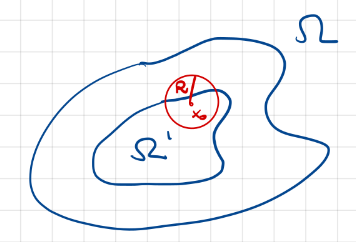
\includegraphics[scale=0.45]{pictures/picture02.png}
	\end{center}
	The general result can then be obtained by a compactness and covering argument (Exercise).\\
	For the case of a ball we need to prove that
	\[ \int\limits_{B_{\frac{R}{2}(x_{0}) }}^{} \abs{\nabla ^{2}u}^{2} \dd{x} \leq c \left( \int\limits_{B_{2R}(x_{0})}^{} \abs{u}^{2} \dd{x} + \int\limits_{B_{2R}(x_{0})}^{} \abs{f}^{2} \dd{x} + \int\limits_{B_{2R}(x_{0})}^{} \abs{\nabla F}^{2} \dd{x} \right) \] for every \( x_{0} \in \Omega' \).
\end{remark}

\begin{proof}
	\( \bullet \)  Assume w.l.o.g that \( x_{0}=0 \) and \( F=0 \). (note that the term \( \sum_{\alpha }^{}\partial_{x_{\alpha }}F_{i}^{\alpha } \) can always be absorbed into \( f \). In fact \( \norm{f+ \operatorname{div}F^{i}}_{2}\leq \norm{f}_{2}+\norm{\nabla F}_{2} \))\\
	\( \bullet \)  Moreover we assume that \( \lambda \) is constant (it is possible to reduce to the general case, see next lectures) \\
	We start observing that the equation in its weak formulation reads as
	\[ \int\limits_{\Omega}^{} \left\langle A \nabla u, \nabla \varphi  \right\rangle  \dd{x} = \int\limits_{\Omega}^{} \left\langle f,\varphi  \right\rangle  \dd{x}, \qquad \forall  \varphi \in  C_{c}^{\infty }(\Omega ; \mathbb{R}) \]
	In order to simplify the notation in the proof we let \( e_{\gamma } \) be a fixed vector and set \( \tau _{h}:= \tau _{h, \gamma  } \) and \( \Delta _{h := \Delta _{h, \gamma }} \).\\
	We take as test function \( \tau _{-h}\varphi  \), for \( h \) small enough and change variables to get
	\[ \int\limits_{\Omega}^{} \left\langle \tau _{h}(A \nabla u), \nabla \varphi  \right\rangle  \dd{x} = \int\limits_{\Omega}^{} \left\langle \tau _{h}f, \varphi  \right\rangle  \dd{x} \]
	subtracting the two previous equations anf dividing by \( h \) we have that (using Leibniz)
	\begin{align}
		  & \int\limits_{\Omega}^{} \frac{1}{h} \left[ \left\langle A \nabla u, \nabla \varphi  \right\rangle  \right]- \left\langle \tau _{h}(A \nabla u), \nabla \varphi  \right\rangle \dd{x}  \\
		= & \int\limits_{\Omega}^{} \left\langle \underbrace{A \nabla u - \tau _{h}(A \nabla u)}_{h}, \nabla \varphi  \right\rangle  \dd{x}  \\
		= & \int\limits_{\Omega}^{} \left\langle \Delta _{h}(A \nabla u), \nabla \varphi  \right\rangle  \dd{x}  \\
		= & \int\limits_{\Omega}^{} \left\langle \tau _{h} A \nabla (\Delta _{h} u), \nabla \varphi \right\rangle  + \left\langle (\Delta _{h}A) \nabla u, \nabla \varphi  \right\rangle \dd{x}  \\
		= & \int\limits_{\Omega}^{} \left\langle \Delta _{h}f, \varphi  \right\rangle  \dd{x},
	\end{align}
	i.e,
	\[ \int\limits_{\Omega}^{} \left\langle (\tau _{h}A) \nabla (\Delta _{h}u)  \right\rangle  \dd{x} = \int\limits_{\Omega}^{} \left\langle \Delta _{h} f, \varphi  \right\rangle  \dd{x} - \int\limits_{\Omega}^{} \left\langle (\Delta _{h}A) \nabla u, \nabla \varphi \right\rangle  \dd{x} \]
	This is the weak formulation of the equation
	\[ - \sum\limits_{\alpha ,\beta ,j}^{} \partial_{x_{\alpha}} \left( {(\tau _{h}A)}_{ij}^{\alpha \beta } \partial_{x_{\beta }} v^{j} \right)= f_{i}' - \sum\limits_{\alpha }^{} \partial_{x_{\alpha }} G_{i}^{\alpha }, \qquad i=1,2,\ldots,m \tag{EQ} \label{EQ} \]
	where \( v= \Delta _{h}u \). \( f'=\Delta _{h}f \) and \( G=-(\Delta _{h}A) \nabla u \). The basic idea now is to use~\eqref{CLI}. A direct application of it would lead to an estimate in terms of the \( L^{2} \) norm of \( f'=\Delta _{h}f \) which we know can be uniformly bounded in \( h \) only if \( f \in H_{loc}^{1}(\Omega )  \) (by the characterization of Sobolev spaces in terms of difference quotients). Since we have only assumed \( f \in L_{loc}^{2}(\Omega) \), we need to proceed carefully and \enquote{adapt} the proof of~\eqref{CLI}. We consider the cut-off function \( \eta \) compactly supported in \( B_{R} \), \( \eta \in [0,1]  \), \( \eta \equiv 1 \) on \( B_{\sfrac{R}{2}} \) and \( \abs{\nabla \eta }\leq \sfrac{4}{R} \). We need test~\eqref{EQ} with \( \varphi := \eta ^{2}\delta _{h}u= \eta ^{2}v \), where \( \abs{h}<\sfrac{R}{2} \). \\
	As in the proof of~\eqref{CLI} we get
	\[ \frac{3 \lambda }{4}\int\limits_{B_{R}}^{} \eta ^{2}\abs{\nabla v}^{2} \dd{x} \leq  \frac{4 \Lambda \varepsilon }{R}\int\limits_{B_{R}}^{} \eta ^{2}\abs{\nabla v}^{2} \dd{x}+ \left( \frac{4 \Lambda }{R \varepsilon }+ \frac{4}{R^{2}}\right) \int\limits_{B_{R}}^{} \abs{v}^{2} \dd{x}	+ \int\limits_{B_{R}}^{} \eta ^{2}v \Delta _{h}f \dd{x} + \left( \frac{1}{\lambda } + 4	 \right) \int\limits_{B_{R}}^{} \abs{G}^{2} \dd{x}. \]
	Choosing \( \varepsilon > 0 \) we absorb \( \frac{4 \Lambda \varepsilon }{R} \int_{B_{R}}^{} \eta ^{2} \abs{\nabla v}^{2} \dd{x} \) in the L.H.S\ and we get that for some constant \( c=c(\lambda , \Lambda , R) > 0 \)
	\begin{gather}
		c \int\limits_{B_{R}}^{} \eta ^{2}\abs{\nabla v}^{2} \dd{x} \leq \underbrace{\int\limits_{B_{R}}^{} \abs{v}^{2} \dd{x}}_{\eqref{004}} + \underbrace{\int\limits_{B_{R}}^{} \eta ^{2} v \Delta _{h}f \dd{x}}_{\eqref{005} } + \underbrace{\int\limits_{B_{R}}^{} \abs{G}^{2} \dd{x}}_{\eqref{006}} \label{003}
	\end{gather}
	We consider the different terms separately. We notice that (see~\eqref{001} in the proof of Lemma~\ref{lemma01})
	\begin{gather}
		\int\limits_{B_{R}}^{} \abs{v}^{2} \dd{x} = \int\limits_{B_{R}}^{} \abs{\Delta _{h} u}^{2} \dd{x} \leq \int\limits_{B_{R+h}}^{} \abs{\nabla u}^{2} \dd{x} \label{004}
	\end{gather}
	The R.H.S\ of the inequality above can be estimated by the~\eqref{CLI}. In fact \( \int_{B_{R+h}}^{} \abs{\nabla u}^{2} \dd{x} \leq \int_{B_{\sfrac{3}{2}R}}^{} \abs{\nabla u}^{2} \dd{x} \) which can be in turn be estimated by~\eqref{CLI} for \( u \) between the balls \( B_{\sfrac{3R}{2}} \) and \( B_{2R} \), with an upper bound of the type we are looking for. Concerning the term~\eqref{005} we have
	\begin{align}
		\label{005} \abs{\int\limits_{B_{R}}^{} \eta ^{2} v \Delta _{h} f \dd{x}} \overset{\text{discrete by I.P.}}{=} & \abs{\int\limits_{B_{R}}^{} - \Delta _{-h} (\eta ^{2} v) f  \dd{x}}  \\
		\overset{\text{Young }p=q=2}{\leq}                                                                             & \widetilde{\varepsilon} \int\limits_{B_{R}}^{} \abs{\Delta _{-h}(\eta ^{2}v)}^{2} \dd{x} + \frac{1}{ \widetilde{\varepsilon}} \int\limits_{B_{R}}^{} \abs{f}^{2} \dd{x} \notag
	\end{align}
	The term \( \int_{B_{R}}^{} \abs{f}^{2} \dd{x} \leq \int_{B_{2R}}^{} \abs{f}^{2} \dd{x} \) is already fine for the estimate we want. For the other term we have
	\begin{align}
		\widetilde{\varepsilon }\int\limits_{B_{R}}^{} \abs{\Delta _{h}(\eta ^{2}v)}^{2} \dd{x} \overset{\text{Corollary of }~\ref{lemma01}}{\leq} & \widetilde{\varepsilon } \int\limits_{B_{h+r}}^{} \abs{\nabla (\eta ^{2}v) }^{2} \dd{x}  \\
		=                                                                                                                                          & c \widetilde{\varepsilon }\int\limits_{B_{R+h}}^{} \abs{(\nabla \eta ^{2})v+\eta ^{2} \nabla v }^{2} \dd{x}  \\
		\overset{\eqref{007}}{\leq}                                                                                                                & c \widetilde{\varepsilon} \left[ \frac{128}{R^{2}} \int\limits_{B_{R+h}}^{} \abs{v}^{2} \dd{x} + 2 \int\limits_{B_{R+h}}^{} \eta ^{4} \abs{\nabla v}^{2} \dd{x} \right]  \\
		\leq                                                                                                                                       & c \widetilde{\varepsilon } 2 \left[ \int\limits_{B_{R+h}}^{} \abs{\nabla \eta ^{2}}^{2} \abs{v}^{2} \dd{x} + \int\limits_{B_{R+h}}^{} \eta ^{4} \abs{\nabla v}^{2} \dd{x} \right]  \\
		\overset{\eqref{008}}{\leq}                                                                                                                & c \widetilde{\varepsilon} \left[ \frac{128}{R^{2}} \int\limits_{B_{R+h}}^{} \abs{v}^{2} \dd{x} + 2 \int\limits_{B_{R+h}}^{} \eta ^{4} \abs{\nabla v}^{2} \dd{x} \right]  \\
		\overset{\eta ^{4}\leq \eta ^{2}}{\leq}                                                                                                    & \frac{128}{R^{2}}\, c \widetilde{\varepsilon } \int\limits_{B_{R+h}}^{} \abs{v}^{2} \dd{x} + 2\,c \widetilde{\varepsilon }  \int\limits_{B_{R+h}}^{} \eta ^{2}\abs{\nabla v}^{2} \dd{x}
	\end{align}
	For~\eqref{007}, see that
	\begin{gather}
		{(a+b)}^{2}= 4{\left( \frac{1}{2}a+\frac{1}{2}b \right)} ^{2} \overset{\text{conv}}{\leq } 4 \left( \frac{1}{2}a^{2}+ \frac{1}{2}b \right) = 2(a^{2}+b^{2}) \label{007}
	\end{gather}
	and for~\eqref{008}, see that
	\begin{gather}
		\abs{\eta }\leq 1, \, \abs{\nabla \eta }\leq \frac{4}{R} \Rightarrow \abs{\nabla \eta ^{2}}^{2}=\abs{2 \eta \nabla \eta }^{2} < {\left( \frac{8}{R} \right)} ^{2} = \frac{64}{R^{2}} \label{008}
	\end{gather}
	The term \( 2 c \widetilde{\varepsilon } \int_{B_{R+h}}^{} \eta ^{2} \abs{\nabla v}^{2} \dd{x} \) can be absorbed in the l.h.s.\ of~\eqref{003} on choosing \( \widetilde{\varepsilon } \) small enough, while the term \( \frac{128c}{R^{2}} \widetilde{\varepsilon } \int_{B_{R+h}}^{} \abs{v}^{2} \dd{x} \) can again be estimated as in~\eqref{004} using~\eqref{CLI}. \\
	We are left with
	\begin{gather}
		\int\limits_{B_{R}}^{} \abs{G}^{2} \dd{x} = \int\limits_{B_{R}}^{} \abs{\Delta_{h}A \cdot \nabla u}^{2} \dd{x} \overset{\text{A is locally Lip}}{\leq } c \int\limits_{B_{R}}^{} \abs{\nabla u}^{2} \dd{x}, \label{006}
	\end{gather}
	hence we can use~\eqref{CLI} again. \\
	We eventually collect all the estimates to find out that we control uniformly as \( h \to 0 \) the term
	\begin{gather}
		\int\limits_{B_{\frac{R}{2}}}^{} \abs{\nabla v}^{2} \dd{x}	= \int\limits_{B_{\frac{R}{2}}}^{} \abs{\nabla \Delta _{h}u}^{2} \dd{x}	= \int\limits_{B_{\frac{R}{2}}}^{} \abs{\Delta _{h} \nabla u}^{2} \dd{x}
	\end{gather}
	Thanks to Lemma~\ref{lemma01} we obtain the control over \( \int_{B_{\frac{R}{2}}}^{} \abs{\partial_{x_{\gamma }}	\nabla u}^{2} \dd{x} \). By the arbitrariness of \( \gamma \) we control \( \int_{B_{\frac{R}{2}}}^{} \abs{\nabla ^{2}u}^{2} \dd{x} \) as claimed.
\end{proof}